% Copyright 2004 by Till Tantau <tantau@users.sourceforge.net>.
%
% In principle, this file can be redistributed and/or modified under
% the terms of the GNU Public License, version 2.
%
% However, this file is supposed to be a template to be modified
% for your own needs. For this reason, if you use this file as a
% template and not specifically distribute it as part of a another
% package/program, I grant the extra permission to freely copy and
% modify this file as you see fit and even to delete this copyright
% notice. 

\documentclass{beamer}

\usepackage[utf8]{inputenc}
\usepackage{float}
\usepackage[font=small]{caption}
\usepackage{amssymb}
\usepackage{pifont}

\setcounter{tocdepth}{1}

% There are many different themes available for Beamer. A comprehensive
% list with examples is given here:
% http://deic.uab.es/~iblanes/beamer_gallery/index_by_theme.html
% You can uncomment the themes below if you would like to use a different
% one:
%\usetheme{Boadilla}
\usetheme{Hannover}
%\usetheme{Singapore}

\title{Notification Processing}

% A subtitle is optional and this may be deleted
\subtitle{Processing of Notifications Produced by Intrusion Detection Systems in CERN's Security Operations Centre}

\author{Amund Faller Råheim}
% - Give the names in the same order as the appear in the paper.
% - Use the \inst{?} command only if the authors have different
%   affiliation.

\institute[NTNU] % (optional, but mostly needed)
{
  Bachelor of Engineering in Computer Science\\
  Norwegian University of Science and Technology
  }
% - Use the \inst command only if there are several affiliations.
% - Keep it simple, no one is interested in your street address.

\date{7th of June 2017}


% Let's get started
\begin{document}

\begin{frame}
  \titlepage
\end{frame}

\begin{frame}{Outline}
  \tableofcontents
  % You might wish to add the option [pausesections]
\end{frame}


\section{Introduction}
\subsection{Supervisors}
\begin{frame}{Supervisors}
\begin{minipage}{0.4\textwidth}
\begin{figure}[H]

\includegraphics[width=0.4\textwidth]{cern_logo.png}
\end{figure}
\end{minipage} \hfill
\begin{minipage}{0.55\textwidth}
\begin{block}{CERN}
Liviu Valsan, \\Computer Security Team
\end{block}
\end{minipage}

\begin{minipage}{0.4\textwidth}
\begin{figure}[H]
\includegraphics[height=0.45\textwidth]{ntnu_logo.png}
\end{figure}
\end{minipage} \hfill
\begin{minipage}{0.55\textwidth}
\begin{block}{NTNU}
Basel Katt, \\Department of Information Security and Communication Technology
\end{block}
\end{minipage}
\end{frame}


\subsection{The Employer}
\begin{frame}{The Employer}

\begin{block}{The European Organisation for Nuclear Research}
\begin{itemize}
    \item Located near Geneva, Switzerland
    \item Thousands of researchers
    \item Worlds largest machine: LHC
    \item Constant computer security threats
\end{itemize}
\end{block}

\begin{block}{The Computer Security Team}
\begin{itemize}
    \item Several sectors of operation at CERN
    \item Threat detection and prevention
\end{itemize}
\end{block}
\end{frame}


\subsection{Definitions}
\begin{frame}{Definitions}
\begin{block}{Terms}
\begin{itemize}
    % \item SOC: Security Operations Centre
    \item Indicator of Compromise (IOC)
    \item Malware Information Sharing Platform (MISP)
    \item MISP event: IOCs + data about a threat
    \item Security Information and Event Management (SIEM)
\end{itemize}
\end{block}
\end{frame}


\subsection{The Project Environment}
\begin{frame}{The Project Environment}
\begin{block}{Background}
\begin{itemize}
    \item Intrusion Detection Systems
    \item 500 GB/day of internet traffic
    \item Notifications (hundreds/day)
    \item Poor value for analyst
\end{itemize}
\end{block}
\end{frame}

% \begin{figure}
%     \centering
%     \includegraphics[width=\textwidth]{the_SOC.png}
%     \label{fig:soc}
% \end{figure}


\subsection{Problem Area}
\begin{frame}{Problem Area}
\begin{block}{Motivation}
Enriching notifications for better response to security threats.

\begin{itemize}
    \item Varying levels of competence of analysts
    \item Time consuming analysis
    \item Context and correlation
    \item Standardising output
    \item Security Information and Event Management
\end{itemize}
\end{block}
\end{frame}


\section{The Project}
\subsection{Functional Requirements}
\begin{frame}{Functional Requirements}
\begin{block}{Project Description}
\begin{itemize}
    \item Interval processing of notifications
    \item Enriched data fields
    \item Aggregated notifications
    \item Raise alerts
\end{itemize}
\end{block}
\end{frame}


\subsection{Enrichment}
\begin{frame}{Enrichment}
\begin{exampleblock}{Data Fields}
\begin{itemize}
    \item IP address $->$ Device name
    \item Device name $->$ Device info
    \item Indicator of compromise $->$ MISP Event
    \item Network connection $->$ Network traffic history
\end{itemize}
\end{exampleblock}
\end{frame}


\subsection{Quality of Service Requirements}
\begin{frame}{Quality of Service Requirements}
\begin{block}{Quality of Service Requirements}
\begin{itemize}
    \item Modularity
    \item Configurability
    \item Reliability and comletability
    \item Integrity
    \item Logging and traceablity
\end{itemize}
\end{block}
\end{frame}


\section{Implementation}
\subsection{Application Architecture}
\begin{frame}{Application Architecture}
\begin{block}{Components}
\begin{figure}
    \centering
    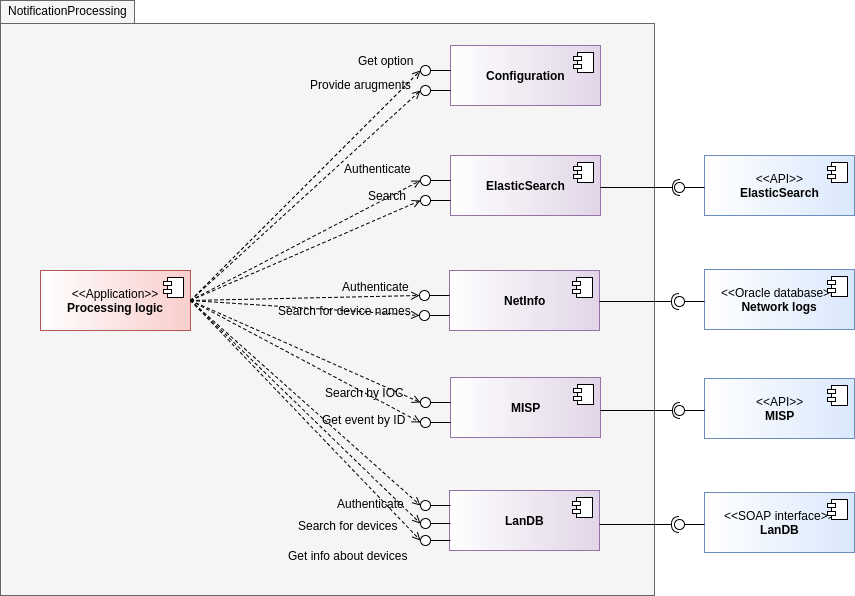
\includegraphics[width=0.9\textwidth]{component-diag.png}
\end{figure}
\end{block}
\end{frame}


\subsection{Tools}
\begin{frame}{Tools}
\begin{block}{}
\begin{itemize}
    \item Python 2.7 for application
    \item Python modules:
    \begin{itemize}
        \item Elasticsearch-py for Elasticsearch
        \item cx\_Oracle for netlog database
        \item PyMISP for MISP
        \item suds for SOAP network database
    \end{itemize}
\end{itemize}
\end{block}
\end{frame}

\subsection{Configuration}
\begin{frame}{Configuration}
\begin{itemize}
    \item Scalable
    \item File
    \item Command line arguments
\end{itemize}

\begin{figure}
    \centering
    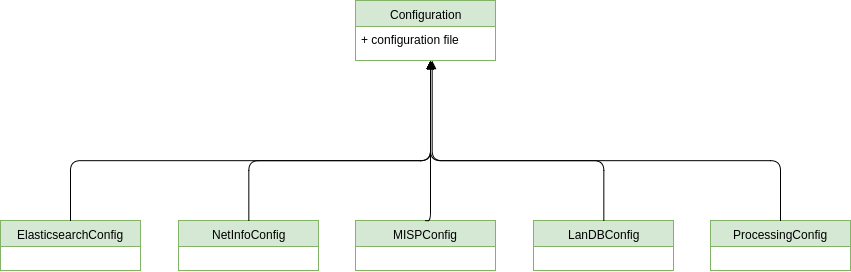
\includegraphics[width=\textwidth]{config.png}
\end{figure}
\end{frame}


\subsection{Finding Correct Device}
\begin{frame}{Finding Correct Device}
\begin{block}{Tricky "NetInfo" module}
\begin{itemize}
    \item ARP and DHCP logs
    \item Time zones
    \item Multiple results
\end{itemize}
\end{block}
\end{frame}


\section{Process}
\subsection{Testing and Code Review}
\begin{frame}{Testing and Code Review}
\begin{block}{Who, why, how}
\begin{itemize}
    \item With CERN supervisor
    \item Approve modules
    \item Optimise logic
    \item Ensure fulfilment of requirements
    \item "Pair programming"
    \item Continuous testing
    \begin{itemize}
        \item Configuration injection
        \item Result analysis
    \end{itemize}
\end{itemize}
\end{block}
\end{frame}


\subsection{Process Evaluation}
\begin{frame}{Process Evaluation}
\begin{block}{Experiences from the process}
\begin{itemize}
    \item Delayed code review
    \item Examine tools in advance
    \item More supervision in start
\end{itemize}
\end{block}
\end{frame}


\section{Conclusion}
\begin{frame}{Conclusion}
\begin{block}{Result}
$ $\: \ding{52} \: Five modules \\
$ $\: \ding{52} \: Correct device name and hardware address \\
$ $\: \ding{52} \: MISP security event \\
$ $\: \ding{52} \: Grouping \\
$ $\: \ding{52} \: Mailing \\
$ $\: \ding{52} \: Configurability \\
$ $\: \ding{52} \: Logging \\
\hfill\\
$ $\: \ding{55} \: Result to database \\
$ $\: \ding{55} \: Related network traffic \\
$ $\: \ding{55} \: Filtering notifications with no network traffic \\
\end{block}
\end{frame}


% Reference to my paper
% \section*{For Further Reading}
\begin{frame}{For Further Reading}
\begin{minipage}{0.8\textwidth}
\begin{thebibliography}{10} 
  \beamertemplatearticlebibitems
  \bibitem{Råheim2017}
    A.F.~Råheim.
    \newblock Processing of Notifications Produced by Intrusion Detection Systems in CERN's Security Operations Centre
    \newblock {\em 2017}

  \end{thebibliography}
\end{minipage}
\end{frame}
\end{document}
